\section{Research Testing}
To provide information about the behaviour of a quadcopter with variable pitch propellers a series of consecutive tests are performed. The characteristics of variable pitch are compared with fixed pitch. The following tests are carried out at KONGSBERG Innovation Center in a confined area. The series of tests are performed with the same physical quadcopter to gain the most comparable datasets. The propellers on the variable pitch quadcopter are fastened at a fixed pitch with a servo actuator, creating a fixed pitch test subject. \\
\\
Having two independent test subjects providing two independent datasets their outcome can be compared. Assuming that the outcome of each of the tests are independent, it is expected that the results will follow normal distribution. When comparing two datasets as described the most common method is the T-test \cite{statistikk}. The T-test is a statistical hypothesis test and it is used to test if the average value of a normalized dataset is significantly different from the null hypothesis and if there is a significant difference between the average values in the two datasets \cite{statistikk2}.\\
\\
The following tests requires that a null hypothesis and an alternative hypothesis are stated. The hypotheses are stated in such a way that they are mutually exclusive. That is, if one is true, the other must be false; and vice versa \cite{statistikk4}. $VPQ_i$ expresses the stochastical variable for the measured value $i$ for dataset 1, $n_1$. $FPQ_j$ expresses the stochastical variable for the measured value $j$ for dataset 2, $n_2$. Assuming that $VPQ_i$ is independent and normal distributed with expectation, $\mu_1$, and standard deviation, $\sigma_1$,  $FPQ_i$ is independent and normal distributed with expectation, $\mu_2$, and standard deviation $\sigma_2$, and $VPQ_i$ are independent from $FPQ_i$. For both dataset the mean and standard deviation are calculated. 
$$H_0:\: \mu_1 = \mu_2 \quad \quad H_1:\: \mu_1 \neq \mu_2$$

%%%%%%%%%%%%%%%%%%%%%%%%%%%%%%%%%%%%%%%
%%%%%%%%%%%%%%%%%%%%%%%%%%%%%%%%%%%%%%%

\subsection{Landing}
To determine if a quadcopter with variable pitch propellers can land more precise than a quadcopter with fixed pitch, a series of consecutive tests must be conducted. From this test we may be able arrive at an indication if variable pitch propellers is able to provide a more precise landing. To determine this the following hypotheses are formulated:\\
\\
$H_0$ = Variable pitch propellers provide the same landing precision as fixed pitch propellers $(\mu_1 = \mu_2 )$\\
$H_1$ = Variable pitch propellers does not provide the same landing precision as fixed pitch propellers $(\mu_1 \neq \mu_2 )$\\

\subsubsection{Test Setup}
In Fig. \ref{fig:landsetup} an illustration of the test setup is displayed. The quadcopter is controlled by a pilot with a Radio Controller and all flights are tracked with the Qualisys Motion Tracking System. To obtain the most comparable data the pilot had to follow the following guidelines:
\begin{enumerate}
  \item Provide throttle for lift in z-axis (above ground effect)
  \item Move forward in y-axis until target position is reached
  \item Land quadcopter as close to the target as possible
\end{enumerate}\\

Four reflective markers are mounted on the quadcopter and . One marker is mounted in the center of the quadcopter, and this marker provides us with the information of how far the quadcopter landed from the target position
\begin{figure}[H]
    \centering
    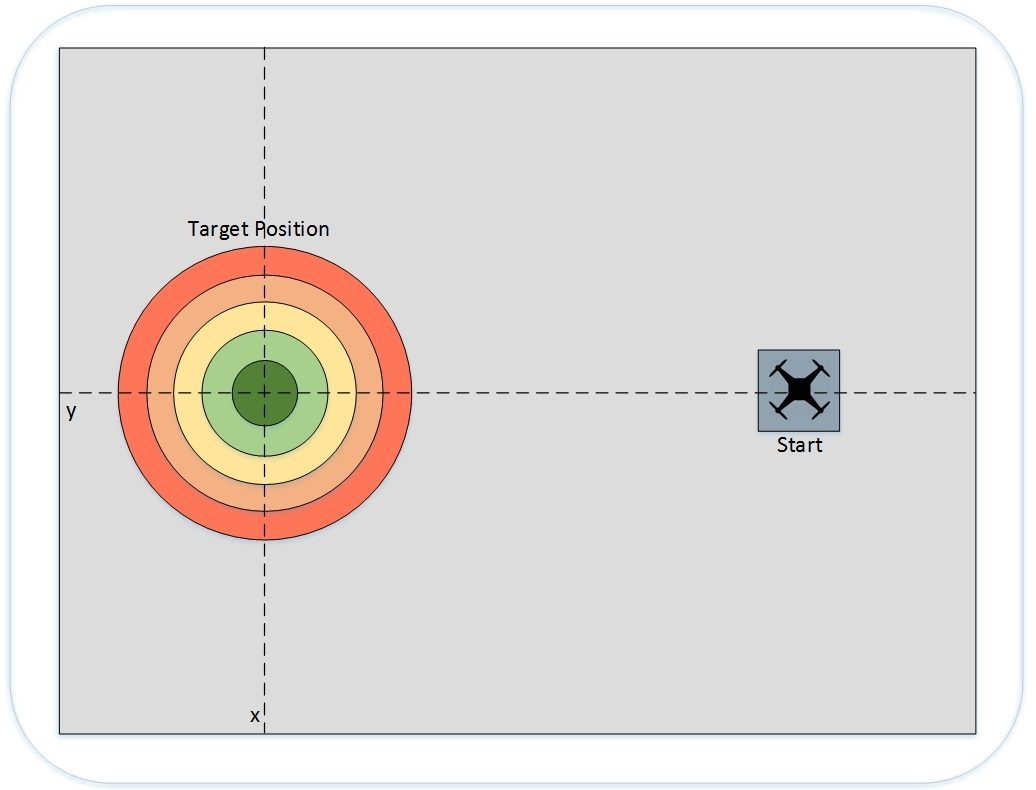
\includegraphics[width = 1\textwidth]{VAPIQ-PICTURES/landingtest}
    \caption{Test Setup for Landing Test}
    \label{fig:landsetup}
\end{figure}

\begin {table}[H]
    \begin{center}
    \caption {Target Position} 
    \label{tab:bla} 
    \begin{tabular}{|l|l|}\hline 
        \textbf{Color:}    & \textbf{Radius [mm]:} \\ \hline
        Green   &  $<$ 25 \\ \hline
        Light Green & $<$ 50 \\\hline
        Yellow & $<$ 75 \\ \hline
        Orange & $<$ 100 \\ \hline
        Red    & $<$ 125 \\ \hline
        Other  & $>$ 150 \\ \hline
        \end{tabular}
    \end{center}
\end{table}

\begin{figure}[H]
    \centering
    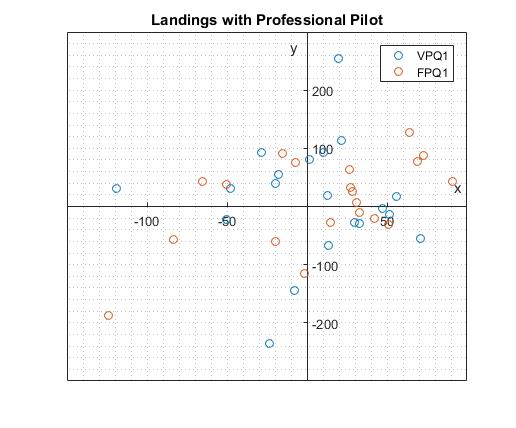
\includegraphics[width = 1\textwidth]{VAPIQ-PICTURES/bothProff}
    \caption{Landing trial 1}
    \label{fig:landsetup2}
\end{figure}

\begin{figure}[H]
    \centering
    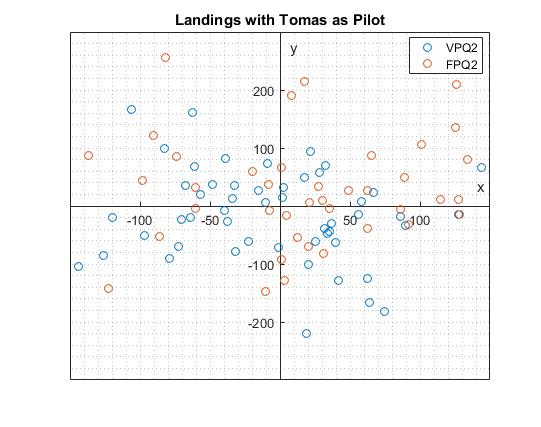
\includegraphics[width = 1\textwidth]{VAPIQ-PICTURES/bothTomas}
    \caption{Landing trial 1 }
    \label{fig:landsetup3}
\end{figure}

\begin{figure}[H]
    \centering
    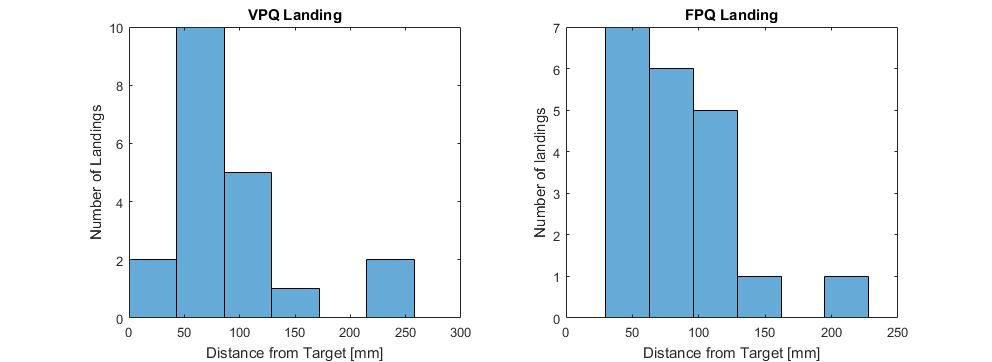
\includegraphics[width = 1\textwidth]{VAPIQ-PICTURES/histoproff}
    \caption{Histogram plot for Professional Pilot}
    \label{fig:landsetup4}
\end{figure}

\begin{figure}[H]
    \centering
    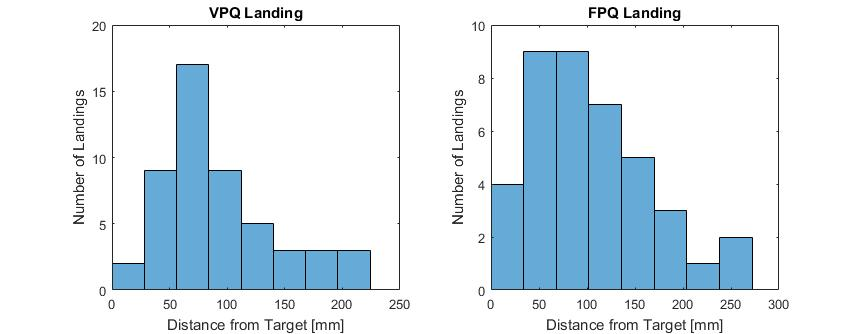
\includegraphics[width = 1\textwidth]{VAPIQ-PICTURES/histotomas}
    \caption{Hstogram plot with Tomas as pilot}
    \label{fig:landsetup}
\end{figure}

\subsubsection*{\textsc{\medium Test Assessment}}
% [Enter a comprehensive assessment of your interpretation of how adequate the test was in light of how thorough the test plan said it should be? What wasn't tested well enough?]
%[Describe any variances between the testing that was planned and the testing that actually occurred.  Also, provide an assessment of the manner in which the test environment may be different from the operational environment and the effect of this difference on the test results
%[Provide a brief description of the unexpected results, problems, or defects that occurred during the testing.]
\subsubsection*{\textsc{\medium Test Results}}


\begin{table}[H]
\caption{Table of Data}
\label{tab:landingdata}
\centering
\begin{tabular}{ l| c c c c} 
     & Mean & Variance & Dataset & Degrees of Freedom\\
 \hline
VPQ & 90.35 & 2802.91   & 71        & 129\\
FPQ & 97.67 & 3369.79   & 60\\
\end{tabular}
\end{table}


\begin{figure}[H]
    \centering
    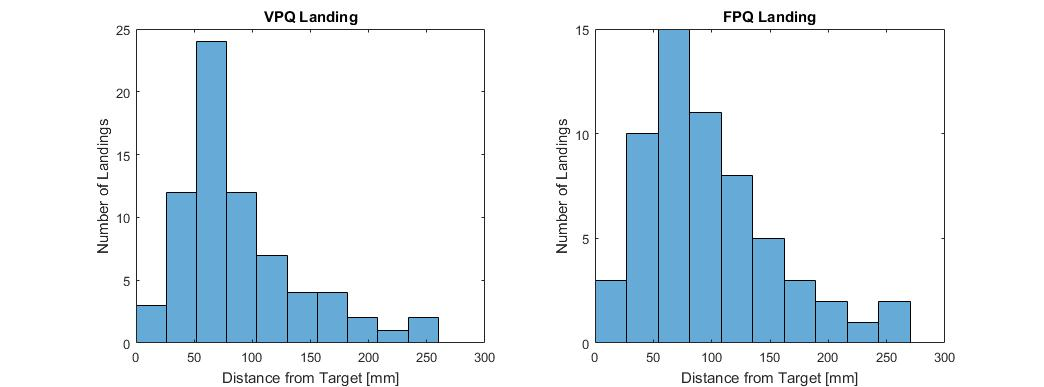
\includegraphics[width = 1\textwidth]{VAPIQ-PICTURES/histoall}
    \caption{Test}
    \label{fig:landsetup}
\end{figure}

\begin{figure}[H]
    \centering
    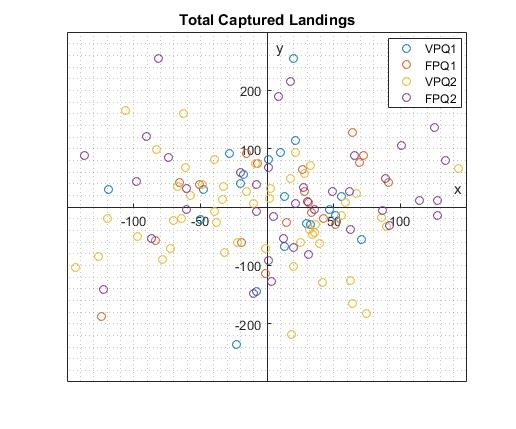
\includegraphics[width = 1\textwidth]{VAPIQ-PICTURES/all}
    \caption{Test}
    \label{fig:landsetup}
\end{figure}


\subsection{Acceleration}
%%%%%%%%%%%%%%%%%%%%%%%
$ H_0$ = Variable pitch propellers provide the same acceleration as fixed pitch propellers $(\mu_1 = \mu_2 )$\\
$ H_1$ = Variable pitch propellers does not provide the same acceleration as fixed pitch propellers $(\mu_1 \neq \mu_2 )$\\
\\\\
%%%%%%%%%%%%%%%%%%%%%%%%%%%%%%%%%%%%%%%

\subsection{Ground Effect}
%%%%%%%%%%%%%%%%%%%%%%%
$H_0$ = A Quadcopter with variable pitch propellers can \\
$H_1$ = A Quadcopter with variable pitch propellers can not 
\\\\
%%%%%%%%%%%%%%%%%%%%%%%%%%%%%%%%%%%%%%%



\begin{comment}
    \subsection{Hover}
    
    http://stattrek.com/hypothesis-test/difference-in-means.aspx?Tutorial=AP
    
    %%%%%%%%%%%%%%%%%%%%%%%
    $H_0$ = A Quadcopter with variable pitch propellers can \\
    $H_1$ = A Quadcopter with variable pitch propellers can not 
    \\\\
    %%%%%%%%%%%%%%%%%%%%%%%%%%%%%%%%%%%%%%%
    histogram
    lager 
    30 stk
    http://www.mn.uio.no/ibv/tjenester/kunnskap/plantefys/matematikk/stat.html#zscore
    %%%%%%%%%%% LOOP 800
    Loop 800 is a measure of the time it takes a propulsion system to increase thrust from 100g to 800g and then decelerate to 400g. It is used to measure the responsiveness of a propulsion system. 
    $H_0$ = A Quadcopter with variable pitch propellers can \\  
    $H_1$ = A Quadcopter with variable pitch propellers can not 
    \\\\
    normaltestplott
    z-axis up and down
    ground effect
    Signifikansnivå?
\end{comment}